\chapter{Introduction} \label{sec:Introduction}

\section{Big Picture} \label{intro:sec:bigpicture}

The discovery of novel materials that solve societal challenges or otherwise improve human lives is arguably one of the most critical components of building a modern world. Starting from the bronze age, humans were able to reliably combine raw materials in a structured fashion to achieve desired results, even though, at the time, there was no mechanistic understanding of \emph{why} things happen. This has changed with gradual introduction of the scientific method, which standardized and systematized the discovery approach, with revolutionary advancements in materials happening every time a new technology for sharing and combining knowledge, such as propagation of the Greek language, printing press, or computer aided design (CAD), has been introduced and widely adopted.

In the current world, which went through the Internet revolution around 2000 and is currently going through the artificial intelligence (AI) revolution of the 2020s, one can point to the informatiztion of materials science as one such communication technology with a potential to revolutionize materials discovery by combining vast amounts of multidimensional data, intricate multidisciplinary domain knowledge, and ability to guide experiments beyond level achievable by a human being. In order to achieve this, one has to consider how to combine these \emph{efficiently}, mitigating problems such as inhomogenities between data sources, computational challenges related to vast design spaces, hidden uncertainties in the reported values, and many flavors of errors, unavoidably present in the complex datasets involved.

While creating an efficient, high-performance, fully general ecosystem for materials informatics appears nearly impossible even for a large group of researchers, a case-specific approach can be constructed in a fashion prioritizing generalizability, which can then be adjusted to other problems. This Dissertation builds such a case-specific approach, embedding a more general blueprint through the development of methods that are rarely limited to the target application but are rather biased towards it through design choices, assumptions, and helpful simplifications. In the process, it introduces several novel individual pieces of software, including \texttt{pySIPFENN}, \texttt{MPDD}, \texttt{crystALL}, \texttt{ULTERA}, \texttt{PyQAlloy}, \texttt{nimCSO}, \texttt{nimplex}, and their derivatives to collectively bridge ab-initio methods, belonging to the domain of quantum physics, with engineering of devices placed in extreme environments, such as gas engine turbine blades or hypersonic vehicles, designed by aerospace engineers, through efficient materials informatics pipelines existing across scales, as summarized in the Figure~\ref{intro:fig:bigpicture} and described in detail in Section~\ref{intro:sec:flow}.

\begin{figure}[H]
    \centering
    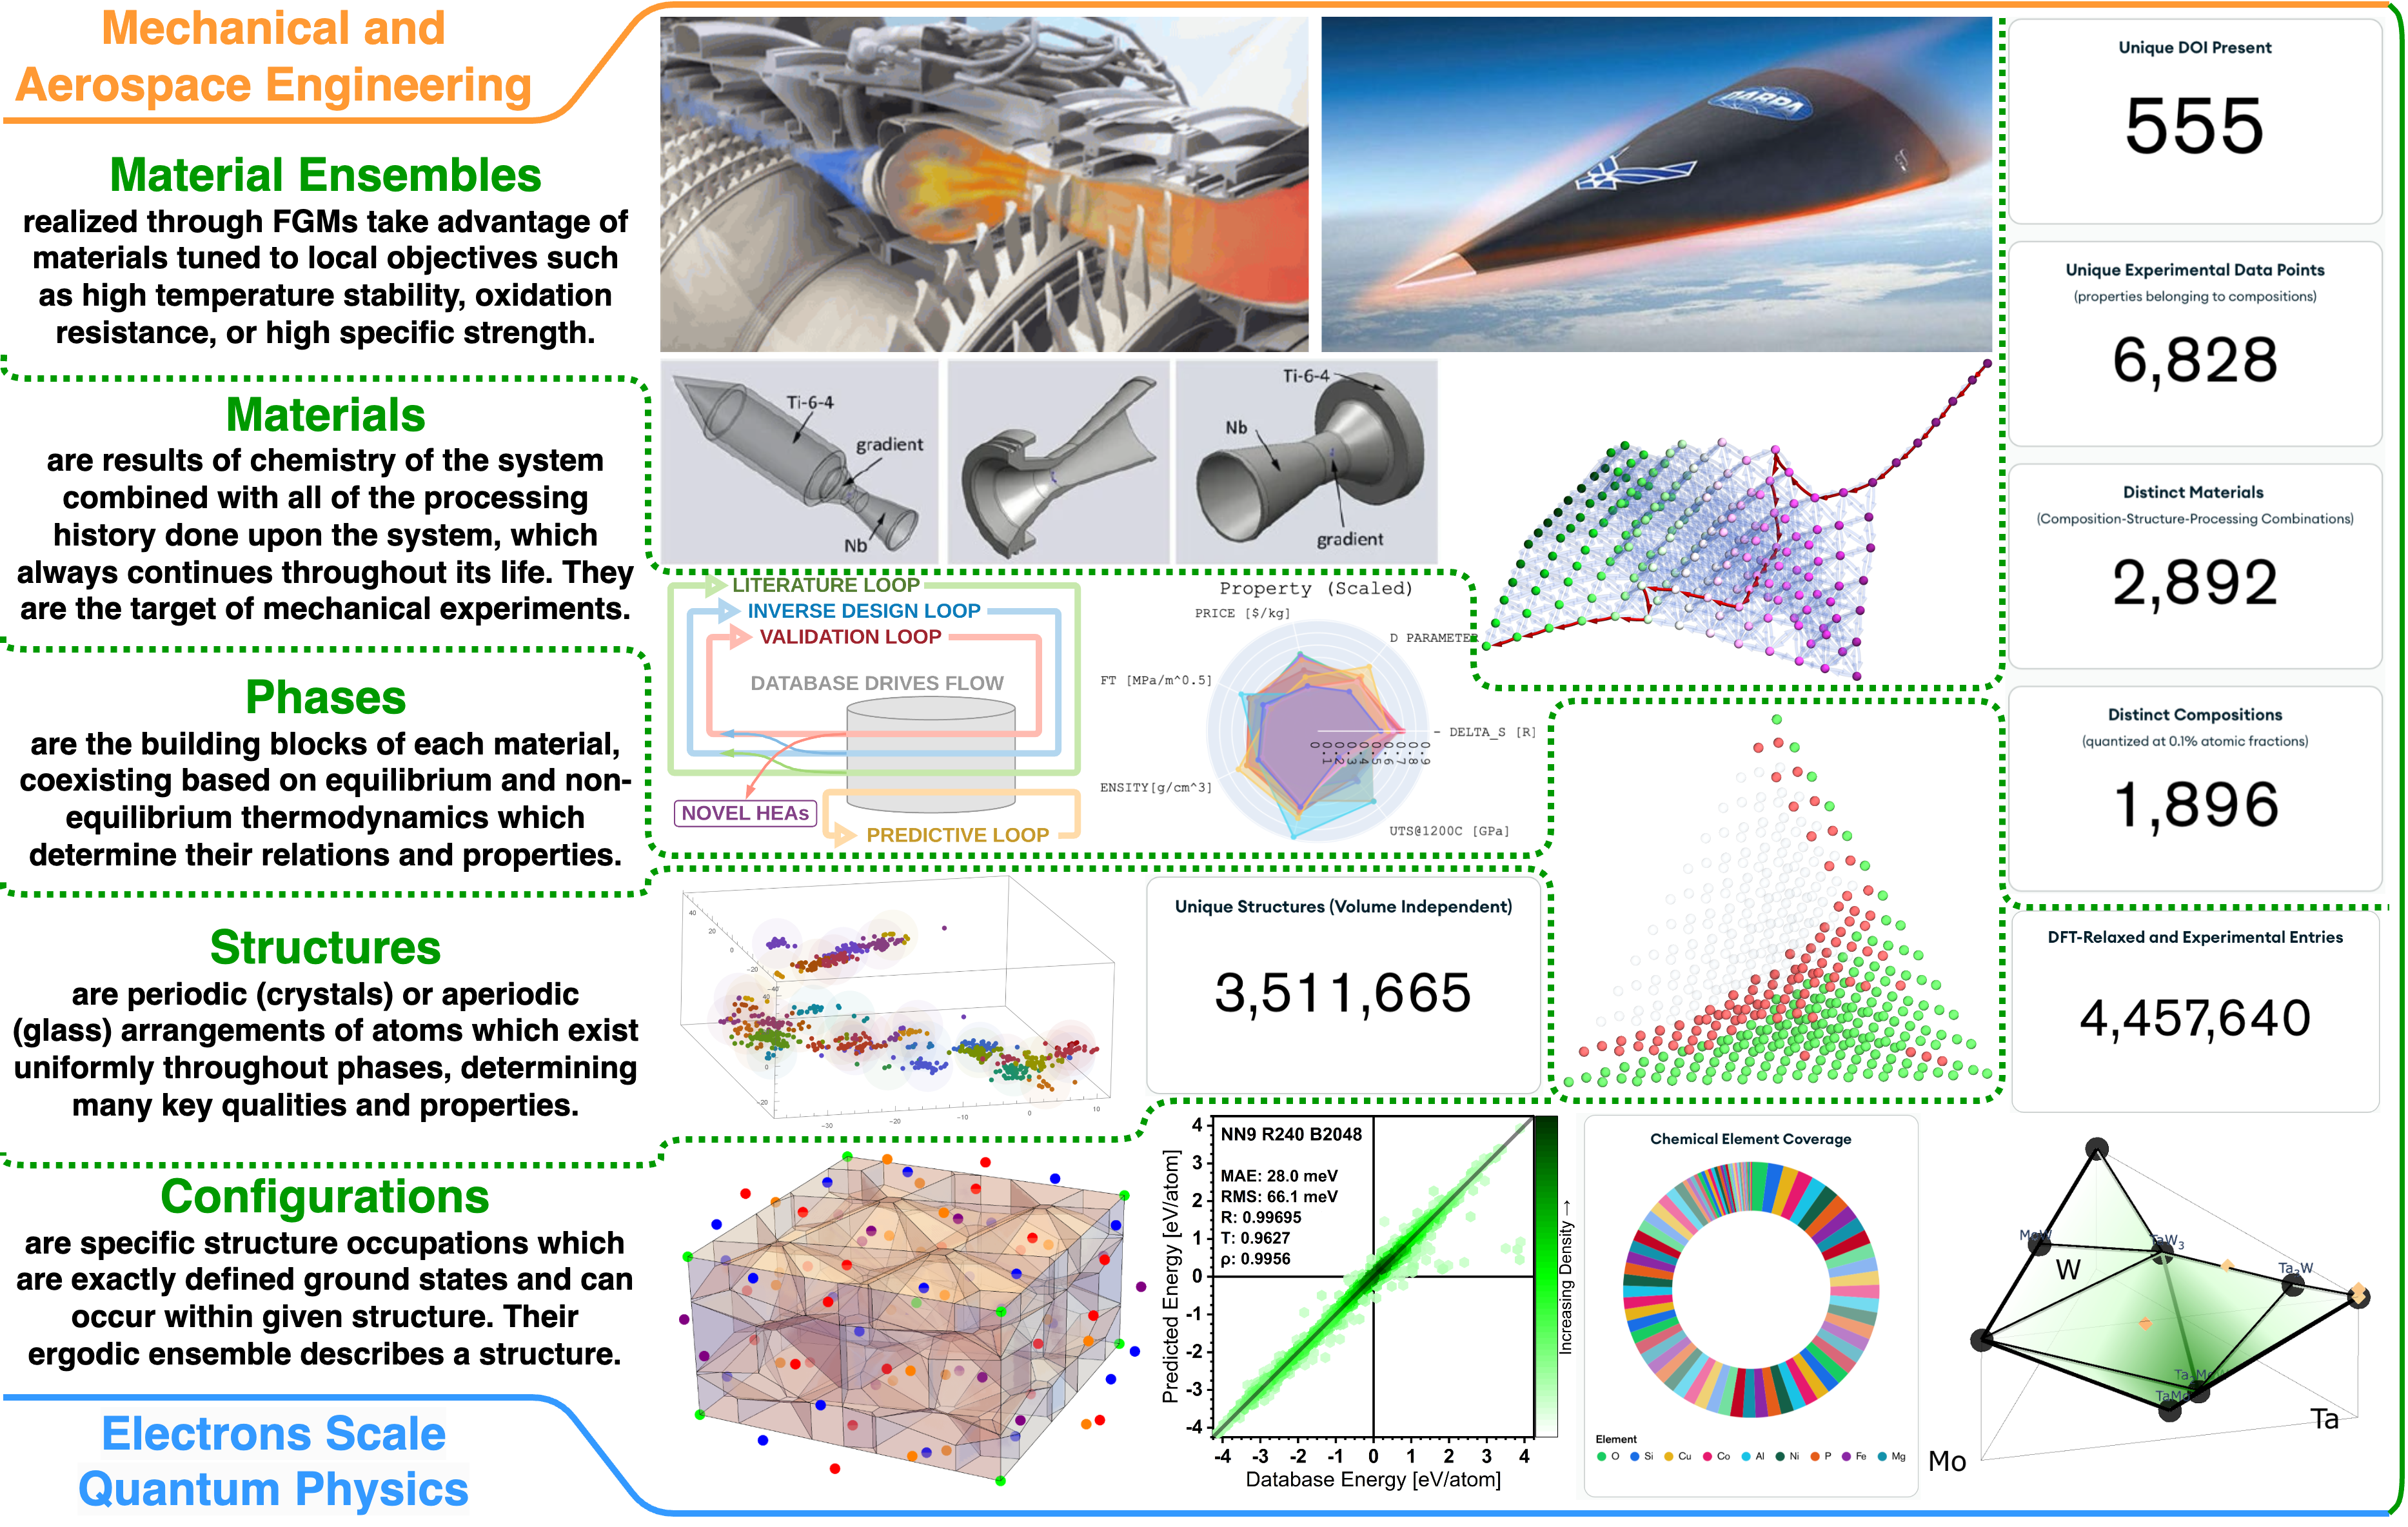
\includegraphics[width=0.95\textwidth]{intro/DissertationBigPicture.png}
    \caption{
    Intermediate material modeling scales bridging together quantum physics and aerospace engineering to enable high-technology solutions through excellence of underlying ensembles of materials. In this work, all of the scales are brought together to take advantage of data and knowledge from all relevant sources. Top render of hypersonic vehicle reproduced from DARPA under public domain and gray nozzle renders from \cite{Hofmann2014DevelopingManufacturing} under CC BY-NC-ND 4.0 License. Several images occur later in the manuscript in Figures \ref{pathplan:fig:lowgradientsquared}, \ref{ultera:fig:dashboard}, \ref{ultera:fig:dataloops}, \ref{inverse:fig:cgandemo}, \ref{infeasibilitygliding:fig:glide}, \ref{crystall:fig:ndbi2clusters}, \ref{pysipfenn:fig:ks2022}, \ref{sipfenn:fig:oqmdperformance}, and \ref{mpdd:fig:dataset}.
    }
    \label{intro:fig:bigpicture}
\end{figure}

The motivation for this specific choice of application - \emph{metallic alloys targeting extreme environments}, has been twofold. First, several intrinsic challenges, including competing property trends, scarce experimental data (relative to room temperature), and compositional complexity of currently studied alloy families, make this problem very difficult. Thus, it is also an excellent target for the design of advanced methods that can mitigate them while encountering and addressing otherwise hidden problems.

- elaborate

Secondly, such alloys are of great interest to the society. For instance, per the US Department of Energy's ARPA-E estimates, developing a standalone alloy that could continuously operate at $1300^oC$ has the potential to increase gas turbine efficiency up to $7\%$, which will significantly reduce wasted energy and carbon emissions by saving up to 20 quads of energy in electricity generation and civilian aviation between now and 2050 \cite{ULTIMATEArpa-e.energy.gov}. Such efficiency increase could prevent the release of approximately 1,000,000,000,000 kg of \ch{CO_2} from burning natural gas, or double that from coal; thus, becoming a critical effort in fighting global warming in applications, like airplanes, where green technologies cannot be directly adapted. Another extreme environment application, quite far from the first one, is the class of hypersonic vehicles that travel faster than 5 times the speed of sound \emph{through Earth's atmosphere for extended periods of time}, thus generating extreme sustained temperatures within structural components. This prompts the need for novel materials and engineering techniques, as evidenced by massive funding assigned to this research area by the US military, which increased its yearly budgets for hypersonic \emph{research} from \$3.8 billion in FY2022 to \$4.7 billion in FY2023, and to an undisclosed amount this year (FY2024) \cite{Sayler2024HypersonicCongress}, further demonstrating the criticality of such materials.

- CHADWICK \cite{CHADWICKArpa-e.energy.gov}

\section{Flow of Material Discovery and This Work} \label{intro:sec:flow}

Throughout this work, all topics raised in Section \ref{intro:sec:bigpicture} will be discussed in a reversed order to progressively build from fundamentals to highly-specialized final applications, while retaining generality at every stage. This way, one will be able to build a holistic picture focused on how data flows within materials informatics research and converges together at consecutive length-scales to discover new materials in specific niches in a systematic, easy-to-automate approach, rather than build elaborate solutions that may \emph{happen} to work well but can also break the fundamentals - a common occurrence in our era of powerful computing and machine learning where tools \emph{always give an answer} but it may hold negative value.

As shown in Figure \ref{intro:fig:outline}, the first 4 chapters (colored blue) cover atomistic treatment of materials, discussing how data at this level is collected, featurized, managed and expanded. \texttt{SIPFENN} approach and the latest \texttt{pySIPFENN} featurization package are first developed. Then \texttt{MPDD} database with 4.5 million DFT-relaxed or experimentally observed entries is set up to serve as a highly efficient deployment vehicle. Lastly, \texttt{crystALL} approach automatically extends it into chemical areas of interest.

\begin{figure}[H]
    \centering
    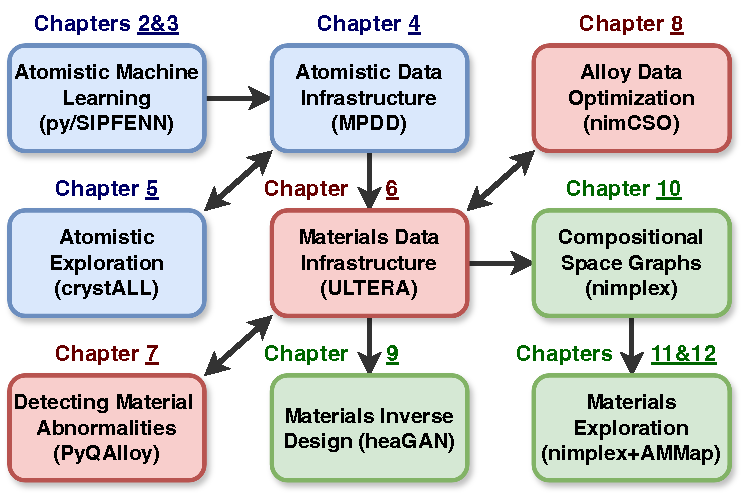
\includegraphics[width=0.7\textwidth]{intro/DissertationOutline.pdf}
    \caption{Schematic outline of this dissertation flowing through 3 overarching types of materials science research. It starts from atomistic treatment (blue) allowing modeling of physical materials (blue) and leading to design (green). For each category, three most significant advancements done in this work have been selected to showcase computational infrastructures and methods to extend our understanding or capabilities.}
    \label{intro:fig:outline}
\end{figure}

All of \texttt{MPDD} is then harvested to model materials at the physical scale by (1) serving as inputs to thermodynamic model generation using \texttt{pycalphad} \cite{Otis2017Pycalphad:Python} and \texttt{ESPEI} \cite{Bocklund2019ESPEICuMg} or training of \texttt{pySIPFENN} ML models generating needed data, and (2) informing experimental observations by, for instance, automatically compiling a set of carbides stable in an alloy system at 0K. At the same time, the largest experimental HEA data infrastructure, called \texttt{ULTERA}, is compiled joining together over 6,800 property datapoints manually extracted from 555 literature publications. 

The experimental database is curated through novel \texttt{PyQAlloy} package created to detect abnormalities and dramatically reduce fraction of erroneous data relative to other similar ones in the literature. Once curated, the \texttt{nimCSO} package can guide ML efforts in terms of which components of the data (chemical elements) should be considered when modeling to optimize trade-off between applicability and data density available to the models. Lastly, compositional space representations generated through \texttt{nimplex} and inverse design workflows serve as deployment vehicles for the trained methods.




\section{Executive Summary} \label{intro:sec:summary}

%%%%%%%%%%
First, Chapter \fullref{chap:sipfenn} introduces fundamental concepts critical to structure-informed modeling of atomic configurations from the perspective of machine learning (ML) modeling and presents design of such models employing artificial neural networks for the prediction of formation energies of atomic structures based on elemental and structural features of Voronoi-tessellated materials. It provide a concise overview of the connection between the machine learning and the true material-property relationship, how to improve the generalization accuracy by reducing overfitting, how new data can be incorporated into the model to tune it to a specific material system, and preliminary results on using models to preform local structure relaxations.

It results in three final models optimized for achieving (1) highest test accuracy on the Open Quantum Materials Database (OQMD), (2) high extrapolative performance in the discovery of new materials, and (3) high performance at a low computational cost. On a test set of 21,800 compounds randomly selected from OQMD, these models achieves a mean absolute error (MAE) of 28, 40, and 42 meV/atom, respectively. The first model represented the state-of-the-art performance on this problem when released in 2020 \cite{Krajewski2020SIPFENNModels} (see Table \ref{sipfenn:comparison-results}), the second model provides better predictions in a test case of interest not present in the OQMD, while the third one reduces the computational cost by a factor of 8 making it applicable to embedded and mobile applications. A transfer learning procedure was also demonstrated for the first time, showing dramatic improvements in extrapolation with just several datapoints (see Figure \ref{sipfenn:fig:transfersigmaVsDatapoints}).

The results were implemented into a new open-source tool called \texttt{SIPFENN} or \textit{Structure-Informed Prediction of Formation Energy using Neural Networks}, which not only improved the accuracy beyond existing models but also shipped in a ready-to-use form with pre-trained neural networks, which was first-of-a-kind at release, and a GUI interface allowing it be included in DFT calculations routines at nearly no cost.


%%%%%%%%
Next, Chapter \fullref{chap:pysipfenn} expands upon \texttt{SIPFENN} and implements a fully-featured machine learning focused analysis framework called \texttt{pySIPFENN} or \textit{python toolset for Structure-Informed Property and Feature Engineering with Neural Networks} to fuel needs of structure-informed materials informatics - a rapidly evolving discipline of materials science relying on the featurization of atomic structures or configurations to construct vector, voxel, graph, graphlet, and other representations useful for machine learning prediction of properties, fingerprinting, and generative design. This chapter discusses how current featurizers typically perform redundant calculations and how their efficiency could be improved by considering (1) fundamentals of crystallographic (orbits) equivalency to optimize ordered cases and (2) representation-dependent equivalency to optimize cases of dilute, doped, and defect structures with broken symmetry. It also discusses and contrasts ways of (3) approximating random solid solutions occupying arbitrary lattices under such representations.

Efficiency improvements discussed in this work were implemented within \texttt{pySIPFENN} and shown to increase performance from 2 to 10 times for typical inputs just based on fundamentals of materials science. Throughout this work, the authors explicitly discuss how these advances can be applied to different kinds of similar tools in the community.


%%%%%%%
Chapter \fullref{mpdd:sec:mpdd} shifts focus from developing new techniques for data analysis to building an innovative atomistic data infrastructure to fuel machine learning model training and deployment process. This effort builds from the idea that, fundamentally, each atomistic ML study comprises of three elements: a dataset or database of \emph{materials}, a \emph{descriptor} or set of features known for each material, and an ML algorithm trained to predict a \emph{property} or a set of them. These three are combined in two steps. First, the data representation is calculated using the descriptor. Then the model is iteratively evaluated on this representation or adjusted to improve it. Both processes are nearly instantaneous compared to ab-initio based methods; however, with extensive databases or materials modeled with large super-cells (e.g., glasses), compute times can grow into days or years for elaborate analysis tools deployed over many millions of datapoints. 

\texttt{MPDD} is a tool that can speed up the total process for the end-user by orders of magnitude through removal of the most time-intensive step, i.e., the descriptor calculation. To accomplish that, it moves from the traditional practice of sharing only the material-properties data to sharing the descriptors-properties data corresponding to the material as well, employing a high-performance NoSQL \texttt{MongoDB} database with highly engineered indexing system and fully salable compute node deployment model. The latter is used to progressively extend it based on guidance received from tools described in later chapters of this dissertation.

\texttt{MPDD} deployment model is not only much faster but also serves as a tool for an automated and robust embodiment of prior knowledge about materials in a graph-like fashion. Lastly, since the descriptors are often reused for related properties, our database provides a tremendous speed-up in the design space exploration.

Since 2023, a stable, well-implemented endpoint of the \texttt{OPTIMADE} API available at \href{https://optimade.mpdd.org}{https://optimade.mpdd.org} allows \texttt{MPDD} to be seamlessly integrated with other community databases and serve atomistic feature data associated with their entries for synergistic merger of experimental observations, ab initio calculations, and machine learning predictions.


%%%%%%%
Chapter \fullref{chap:crystall}, introduces a simple yet powerful approach to discovery of new atomic structures and identification of experimentally observed ones that evade identification, which was already demonstrated in certain important chemical systems. It implements in a concise computational tool which leverages millions of previously calculated structures from \texttt{MPDD} Database and other databases accessed through the \texttt{OPTIMADE} API to identify all atomic structures that can accommodate target stoichiometry (or uncertain chemical composition form experiments) and perform all permutations of substitutions to arrive at a list of tens of thousands of candidate structures. 

It analyzes candidates in the \texttt{KS2022} feature space, introduced in Chapter \ref{chap:pysipfenn} as part of \texttt{pySIPFENN}, to detect unique set of structures underlying different atomic configurations through different clustering techniques. Lastly, it selects a member from each cluster based on minimum formation energy to arrive at an ensemble of candidate configurations then passed to ab initio calculations or experiments for validation. 

Such ensemble approach is shown to provide critical advantages when contrasted with convex-hull-structure searching approach which recently dominated the community. It can also be used to expand unexplored regions of \texttt{MPDD} database, providing valuable deployment target for machine learning models.


%%%%%%%
Chapter \fullref{chap:ultera} crosses from the atomistic-level materials science into "real" materials physically created and measured experimentally, while still focusing on similar aspects of efficient modeling, data handing, and model deployment. It discusses the \texttt{ULTERA} Database, developed under the ARPA-E's ULTIMATE program and aimed at collecting literature data on high entropy alloys (HEAs).

\texttt{ULTERA} facilitates rapid discovery of new alloys using forward and inverse design, with the primary focus on creep behavior, yield stress, ductility, and hardness. Its advanced architecture, composed of many intermediate databases, pipelines, and analysis tools, is designed to automatically integrate starting literature data in real-time with methods such as experiments, generative modeling, predictive modeling, and validations. Thanks to such automation, the experimental team can operate on the best candidates available, while generation of new ones based on incoming experiments can be delegated to the cloud.

As of April 2024, ULTERA contains over 6,800 property-datapoints, corresponding to 2,900 unique HEAs, manually collected from 550 source literature publications. All data is available through a high-performance API, following FAIR principles.


%%%%%%%
Chapter \fullref{chap:pyqalloy} takes the \texttt{ULTERA} Database and dramatically increases its value to the machine learning applications by removing or fixing approximately 5\% of the errors present in it and other state-of-the-art HEA datasets, arriving at \emph{several times less erroneous data}.

In the past, these challenge was not as severe nor impactfull because the effort placed in the data analysis was much greater than data extraction; however, as our community moves towards this large-scale multi-source data collection, it increasingly starts to surface impacting ML efforts. While present in datasets on all alloy classes, this problem is particularly visible in high entropy alloys (HEAs) due to their novelty and complexity. A number of factors causes errors, including a lack of standardized notations and general parsing mistakes, such as typos, but most of them can be caught through detection of abnormalities in relation to the correct data and its patterns.

In this chapter, we present an open-source Python tool called \texttt{PyQAlloy} that can be run on alloy datasets to screen them for a variety of such abnormalities. It puts each data point in a variety of scopes ranging from individual datapoint analysis, through single-study meta-data, to the database as a whole.


%%%%%%%
Chapter \fullref{chap:nimcso} builds on top of \texttt{ULTERA} datasets curated by \texttt{PyQAlloy} and recognizes that selecting dimensions to model, or in this case, the selection of chemical elements to restrict the modeling effort, is a combinatorically hard problem for complex compositions existing in highly dimensional spaces due to the interdependency of components being present. Consequentially, optimizing the data availability and density for applications such as machine learning becomes a challenge.

A novel tool, called \texttt{nimCSO}, has been introduced and implmenets several methods for performing this task over even millions of datapoints and extreme dimensionalities encountered, for instance, in materials science of Compositionally Complex Materials (CCMs) which often span 20-45 chemical elements, 5-10 processing types, and several temperature regimes, for up to 60 total data dimensions.

It achieves the extreme performance by leveraging the metaprogramming ability of the Nim language to optimize itself at the compile time, both in terms of speed and memory handling, to the specific problem statement and dataset at hand based on a human-readable configuration file. As demonstrated in the chapter, it reaches the physical limits of the hardware (L1 cache latency) and can outperform an efficient native Python implementation over 400 times in terms of speed and 50 times in terms of memory usage (\emph{not} counting interpreter), while also outperforming NumPy implementation 35 and 17 times, respectively, when checking a candidate solution. It was designed to be both a user-ready tool and a scaffold for building even more elaborate methods in the future, including heuristics going beyond data availability. 


%%%%%%%
Chapter \fullref{chap:inversedesign} demonstrates how \texttt{ULTERA} dataset can be used to propose new alloys through inverse design. It leverages conditional Generative Adversarial Netowrks (cGAN) models to bias the predicted alloys in terms of (1) the property values by setting the conditioning and (2) the predicted compositions by recognizing \emph{concept vectors} in the latent space established at the training step. The former ability is implemented within a demonstrator Python package called \texttt{heaGAN} which can be used to design HEAs by setting design criteria. It also allows advanced users to re-train cGAN models based on their own data or a third-party property surrogate model.

%%%%%%%
Chapter \fullref{chap:nimplex} departs from both data and machine learning to focus on the mathematical abstractions of the alloy design problem. It begins by considering that many disciplines of science and engineering deal with problems related to compositions, ranging from chemical compositions in materials science to portfolio compositions in economics. They exist in non-Euclidean simplex spaces, causing many standard tools to be incorrect or inefficient, which is significant in combinatorically or structurally challenging spaces exemplified by Compositionally Complex Materials (CCMs) and Functionally Graded Materials (FGMs). In this chapter, we explore them conceptually in terms of problem spaces and quantitatively in terms of computational feasibility.

Several essential methods specific to the compositional (simplex) spaces are implemented, with most critical parts presented in chapter body as code listings, through a high-performance open-source library \texttt{nimplex}. Most significantly, we derive and implement an algorithm for constructing a novel n-dimensional simplex graph data structure, which contains all discretized compositions and all possible neighbor-to-neighbor transitions as pointer arrays. Critically, no distance or neighborhood calculations are performed, instead leveraging pure combinatorics and the ordering in procedurally generated simplex grids, keeping the algorithm $\mathcal{O}(N)$, so that graphs with billions of transitions take seconds to construct on a laptop. Furthermore, we demonstrate how such graph representations can be combined to express path-planning problem spaces and to incorporate prior knowledge while keeping the problem space homogeneous. This allows for efficient deployment of existing high-performance gradient descent, graph traversal search, and other path optimization algorithms.


%%%%%%%
Chapter \fullref{chap:infeasibilitygliding} leverages the novel graph-based representations of compositional spaces to dramatically improve our approach to screening and modifying compositionally complex alloys based on their structural constraint feasibility. It builds on the fact that the equilibrium existence of a particular phase in the phase-regions of chemical space (not necessarily corresponding to the present elements, as exploted in Chapter \ref{chap:nimplex}) is bound by a continuous surface of (generally) low curvature. Thus, performing the community-standard brute force screening type evaluation of all compositions will often calculate high numbers of points that cannot be reached.

Thus, \texttt{nimplex}-generated graphs are used to quickly re-implement the screening procedure into depth-first search traversals of the feasible regions that \emph{glide one the infeasibility boundaries}, reducing computation by half in semi-randomly picked "bad-case" which was known to produce relatively large feasible regions. In more elaborate screenings not taking advantage of prior knowledge, this improvement may very well reach between one and several orders of magnitude.


%%%%%%%
Lastly, Chapter \fullref{chap:pathplanning} takes additional advantage of the \texttt{nimplex}-generated graphs, which can be also extracted from feasible regions established in \ref{chap:infeasibilitygliding}, to deploy path planning algorithms and find sets of compositions that allow dissimilar alloys to be continuously combined in the least number of steps. Additional considerations are made in relation to an example property field of Root Mean Square Atomic Displacement (RMSAD) related to the yield stress in HEAs. In particular, its value, gradient, and magnitude of gradient are used to modify the graph weights encoding different design objectives, which are effortlessly solved with the same out-of-the box pathfinding approach.


%%%%%%%
Appendix \fullref{chap:supdiscussions} explores minor considerations tangential to the information flow or otherwise less critical, that may be of significant interest to some readers, while Appendix \fullref{chap:othersoft} discusses 8 pieces of software developed to during this work bur (1) were not directly used, (2) critical to discussion, or (3) were a contribution of a component to existing software.

Appendices \fullref{chap:nimplextutorial1} and \fullref{chap:nimplextutorial2} contain workshop material available under \texttt{nimplex} repository adapted to the formatting of this dissertation and go into details of both "Why?" and "How?" tools introduced between Chapters \ref{chap:nimplex} and \ref{chap:pathplanning} can be used by the end user. They can be run interactively with one-click cloud virtual environment by following current link at \href{https://nimplex.phaseslab.org}{nimplex.phaseslab.org} or by running them locally based on the supplementary materials.

Appendices \fullref{chap:pysipfenntutorial1} and \fullref{chap:pysipfenntutorial2} showcase how \texttt{pySIPFENN} integrates with other computational tools in the community and enables one to guide remote DFT calculations on a server cluster and adjust its models to a specific problem. Both were given by Adam Krajewski as guest lectures in the MatSE 580 course at Penn State in the Fall of 2023 and can be run interactively with one-click cloud virtual environment by following current link at \href{https://amkrajewski.github.io/MatSE580GuestLectures}{amkrajewski.github.io/MatSE580GuestLectures}, which also neatly presents the expected outcomes, or by running them locally based on the supplementary materials.

\printbibliography[heading=subbibintoc]